\documentclass[10pt]{article}

\usepackage{amsmath, amssymb, mathtools}
\usepackage{tikz}
\usetikzlibrary{decorations.markings}
\usepackage[margin=1.5cm]{geometry}

\input prettyprint
\input preamble
\input pdfmsym

\pdfmsymsetscalefactor{10}
\initpps

\def\pmat#1{\begin{pmatrix} #1 \end{pmatrix}}

\let\divides=\mid
\newfunc{det}{{\rm det}}({})
\newfunc{metric}\rho({})
\newfunc{metricc}\sigma({})
\newfunc{spa}{{\rm span}}(\vert)
\newfunc{diam}{{\rm diam}}(\vert)
\newfunc{proj}\pi({})
\newfunc{iproj}{\pi^{-1}}({})
\newfunc{cis}{{\rm cis}}({})
\newfunc{Re}{{\rm Re}}({})
\newfunc{Im}{{\rm Im}}({})
\newfunc{sup}{{\rm sup}}\{\vert\}
\newfunc{Res}{{\rm Res}}({})
\newfunc{wind}n({})
\newfunc{pv}{{\rm pv}}({})
\newfunc{lspan}{{\rm span}}\{|\}
\newfunc{spec}{{\rm spec}}({})
\newfunc{trace}{{\rm trace}}({})

\font\bigbf = cmbx12 scaled 2000
\@undervecc@def{underbar}\@linecap\@linecap

\def\pmat#1{\begin{pmatrix}#1\end{pmatrix}}

\def\mO{{\cal O}}
\def\mU{{\cal U}}
\let\lineseg=\overleftrightvecc
\let\to=\varrightarrow
\let\longto=\longvarrightarrow
\let\ds=\displaystyle

\def\pdv#1#2{\frac{\partial #1}{\partial #2}}

\def\differ#1#2{\left.d#1\strut\right|_{#2}}

\def\qed{%
    \ifmmode%
        \eqno\blacksquare%
    \else%
        \hskip1cm\allowbreak\hbox{}\nobreak\hfill$\blacksquare$%
    \fi%
}

\def\@ppmathcount{\thesection.\thepp@mathcount}

\def\bexerc{\begin{exercise*}}
\def\eexerc{\end{exercise*}}
\def\bblank{\begin{blankpp}}
\def\eblank{\end{blankpp}}

\begin{document}

\c@section=3

\barcolorbox{220, 255, 220}{0, 130, 0}{80, 200, 80}{
    \leftskip=0pt plus 1fill \rightskip=\leftskip
    {\bigbf Differential and Analytic Geometry}

    \medskip
    \textit{Assignment \thesection}

    \textit{Ari Feiglin}
}

\bigskip

\bexerc

    Simplify the following expressions using Einstein notation.
    Assume that all vectors are in $\bR^3$ and all matrices are in $M_3(\bR)$.
    \benum
        \item $\delta^a_bg_{ca}g^{bd}\delta^c_d$
        \item $\delta^i_jg_{ik}\delta^k_m$
        \item $\delta_{ij}a^{ij}$
        \item $g^{1a}g_{a1}$
        \item $\delta^1_a\delta^a_b\delta^b_c\delta^c_d\delta^d_2$
    \eenum

\eexerc

\bblank

    \benum
        \item Here every index occurs both as a lower and upper index, and thus all indexes are being summed over.
        Since $\delta^a_bg_{ca}=g_{cb}$ and $g^{bd}\delta^c_d=g^{bc}$, we get that this is equal to $g_{cb}g^{bc}$, which is the product of a matrix and its inverse at the index $c,c$.
        So this is equal to $\delta^c_c$, which again gets summed over and since $\delta^c_c=1$ for a specific $c$, and the size of each matrix is $3\times3$, this is equal to
        \[ \sum_{c=1}^3\delta^c_c = 3 \]
        Thus the expression is equal to $3$.

        \item Here, $j$ and $m$ only occur as lower indexes and so they are free.
        All other indexes are summed over.
        Since $\delta^i_jg_{ik}=g_{jk}$, this is equal to $g_{jk}\delta^k_m=g_{jm}$.

        \item Here all the indexes are summed over.
        And $\delta_{ij}a^{ij}=a^{ii}$, and so this is equal to $a^{11}+a^{22}+a^{33}$ which is equal to the trace of $A^{-1}$ (the trace of the inverse of $(a_{ij})$).

        \item Here the only index is $a$ and it is summed over (the other index is constant).
        $g^{1a}g_{a1}=\delta^1_1=1$ ($a^{ij}b_{jk}$ is equal to the product of $AB$ at the index $i,k$).

        \item All indexes here are summed over (other than the constants).
        And so
        \[ \delta^1_a\delta^a_b\delta^b_c\delta^c_d\delta^d_2 = \delta^1_b\delta^b_c\delta^c_2 = \delta^1_c\delta^c_2 = \delta^1_2 = 0 \]
    \eenum

\eblank

\bexerc

    Prove the following results using Einstein notation.
    \benum
        \item Let $A$ and $B$ be matrices in $M_n(\bR)$, then $\traceof{AB}=\traceof{BA}$.
        \item Let $A\in M_{n\times m}(\bR)$, $B\in M_{m\times k}(\bR)$, and $C\in M_{k\times\ell}(\bR)$, then $A(BC)=(AB)C$.
    \eenum

\eexerc

\bblank

    \benum
        Let $C=AB$ and $D=BA$, our goal is to show that $\traceof C=\traceof D$.
        Now,
        \[ \traceof C = c^i_i = a^i_jb^j_i \]
        and
        \[ \traceof D = d^j_j = b^j_ia^i_j = a^i_jb^j_i = \traceof C \]
        as required.

        \item Let us define
        \[ D=AB,\quad E=(AB)C,\quad F=BC,\quad G=A(BC) \]
        our goal is to show that $E=G$.
        Now, we know that $d^i_j=a^i_kb^k_j$ and $f^i_j=b^i_kc^k_j$ and so
        \[ e^i_j = d^i_kc^k_j = a^i_\ell b^\ell_k c^k_j \]
        and
        \[ g^i_j = a^i_\ell f^\ell_j = a^i_\ell b^\ell_k c^k_j = e^i_j \]
        Thus we have that $G=E$ as required.
    \eenum

\eblank

\bexerc

    Find a parameterization for a cone, as a rotational surface about $z$.
    And find the metric for this parameterization.

\eexerc

\bblank

    The curve which defines the surface is $\beta(t)=(t,0,t)$.
    Then the surface is parameterized by
    \[ \sigma(\theta,t) = (t\cos\theta,t\sin\theta,t) \]
    Then $\sigma_1=(-t\sin\theta,t\cos\theta,0)$ and $\sigma_2=(\cos\theta,\sin\theta,1)$.
    By definition $g_{ij}=\iprod{\sigma_i,\sigma_j}$ and so
    \begin{gather*}
        g_{11} = t^2\sin^2\theta+t^2\cos^2\theta = t^2 \\
        g_{12} = g_{21} = -t\sin\theta\cos\theta + t\cos\theta\sin\theta = 0 \\
        g_{22} = \cos^2\theta+\sin^2\theta+1 = 2
    \end{gather*}
    Thus the metric is
    \[ g = \pmat{t^2 & 0 \\ 0 & 2} \]

\eblank

\bexerc

    Find the metric of the surface $\sigma(u,v)=(u\cos v,u\sin v,v)$.

\eexerc

\bblank

    First we compute the partial derivatives of $\sigma$.
    \begin{align*}
        \sigma_1(u,v) &= (\cos v,\sin v,0) \\
        \sigma_2(u,v) &= (-u\sin v,u\cos v,1)
    \end{align*}
    And since $g_{ij}=\iprod{g_i,g_j}$ we get
    \begin{gather*}
        g_{11} = \cos^2 v+\sin^2 v = 1 \\
        g_{12} = g_{21} = -u\cos v\sin v + u\cos v\sin v = 0 \\
        g_{22} = u^2\sin^2v + u^2\cos^2v + 1 = u^2 + 1
    \end{gather*}
    And so the metric is
    \[ g = \pmat{1 & 0 \\ 0 & u^2 + 1} \]

\eblank

\bexerc

    \benum
        \item Find the parameterization for the catenoid defined as the rotational surface of $(\cosh\phi,0,\phi)$ about the $z$ axis.
        \item Find the metric for the catenoid.
    \eenum

\eexerc

\bblank

    \benum
        \item Rotational surfaces of curves of the form $(r(\phi),0,z(\phi))$ are $\sigma(\theta,\phi)=(r(\phi)\cos\theta,r(\phi)\sin\theta,z(\phi))$, as this is the result of multiplying $R_\theta$ by them,
        where
        \[ R_\theta = \pmat{\cos\theta & -\sin\theta & 0 \\ \sin\theta & \cos\theta & 0 \\ 0 & 0 & 1} \]
        So the parameterization is
        \[ \sigma(\theta,\phi) = (\cosh(\phi)\cos\theta,\cosh(\phi)\sin\theta,\phi) \]

        \item Once again, we find $\sigma$'s partial derivatives:
        \begin{align*}
            \sigma_1(\theta,\phi) &= (-\cosh(\phi)\sin\theta,\cosh(\phi)\cos\theta,0) \\
            \sigma_2(\theta,\phi) &= (\sinh(\phi)\cos\theta,\sinh(\phi)\sin\theta,1)
        \end{align*}
        And since $g_{ij}=\iprod{\sigma_1,\sigma_2}$ we get
        \begin{align*}
            g_{11} &= \cosh(\phi)^2 \\
            g_{12} = g_{21} &= 0 \\
            g_{22} &= \sinh(\phi)^2 + 1
        \end{align*}
        And so
        \[ g = \pmat{\cosh(\phi)^2 & 0 \\ 0 & \sinh(\phi)^2 + 1} \]
    \eenum

\eblank

\bexerc

    \benum
        \item Find a parameterization for the rotation of the ellipse
        \[ 2x^2 + 3(z-4)^2 = 5 \]
        about the $z$ axis.
        \item Find the metric for this parameterization.
    \eenum

\eexerc

\bblank

    \benum
        \item The ellipse itself can be parameterized by
        \[ \beta(\phi) = \parens{\sqrt{\frac52}\cos\phi,0,\sqrt{\frac53}\sin\phi+4} \]
        And so the rotation is
        \[ \sigma(\theta,\phi) = \parens{\sqrt{\frac52}\cos\phi\cos\theta,\,\sqrt{\frac52}\cos\phi\sin\theta,\,\sqrt{\frac53}\sin\phi+4} \]

        \item Again, we find the partial derivatives of $\sigma$,
        \begin{align*}
            \sigma_1 &= \parens{-\sqrt{\frac52}\cos\phi\sin\theta,\,\sqrt{\frac52}\cos\phi\cos\theta,\,0} \\
            \sigma_2 &= \parens{-\sqrt{\frac52}\sin\phi\cos\theta,\,-\sqrt{\frac52}\sin\phi\sin\theta,\,\sqrt{\frac53}\cos\phi}
        \end{align*}
        And using $g_{ij}=\iprod{\sigma_i,\sigma_j}$ we get
        \begin{align*}
            g_{11} &= \frac52\cos^2\phi \\
            g_{12} = g_{21} &= 0 \\
            g_{22} &= \frac53 + \frac56\sin^2\phi
        \end{align*}
        So the metric is
        \[ g = \pmat{\frac52\cos^2\phi & 0 \\ 0 & \frac53 + \frac56\sin^2\phi} \]
    \eenum

\eblank

\bexerc

    Let us focus on the rotation surface of the parabola $x=z^2+\frac14$ around the $z$ axis.
    \benum
        \item Find the first and second fundamental forms of the surface.
        \item Find the shape operator of the surface.
        \item Find the Gaussian and mean curvature of the surface.
    \eenum

\eexerc

\bblank

    Firstly, the curve (parabola) is given by
    \[ \beta(\phi) = \parens{\phi^2+\frac14,0,\phi} \]
    and so the rotation surface is
    \[ \sigma(\theta,\phi) = \parens{\parens{\phi^2+\frac14}\cos\theta,\,\parens{\phi^2+\frac14}\sin\theta,\,\phi} \]
    And so the first and second partial derivatives of $\sigma$ are:
    \begin{align*}
        \sigma_1 &= \parens{-\parens{\phi^2+\frac14}\sin\theta,\,\parens{\phi^2+\frac14}\cos\theta,\,0} \\
        \sigma_2 &= \parens{2\phi\cos\theta,\,2\phi\sin\theta,\,1} \\
        \sigma_{11} &= \parens{-\parens{\phi^2+\frac14}\cos\theta,\,-\parens{\phi^2+\frac14}\sin\theta,\,0} \\
        \sigma_{22} &= \parens{2\cos\theta,\,2\sin\theta,\,0} \\
        \sigma_{12} &= \parens{-2\phi\sin\theta,\,2\phi\cos\theta,\,0}
    \end{align*}

    \benum
        \item We know that the first fundamental form is given by $g_{ij}=\iprod{\sigma_i,\sigma_j}$.
        So
        \begin{align*}
            g_{11} &= \parens{\phi^2+\frac14}^2 \\
            g_{12} = g_{21} &= 0 \\
            g_{22} &= 4\phi^2 + 1
        \end{align*}
        And so the first fundamental form is
        \[ g = \pmat{\parens{\phi^2+\frac14}^2 & 0 \\ 0 & 4\phi^2 + 1} \]

        Now let us find the unit normal vector to the surface.
        Recall that this is given by
        \[ \rho = \frac{\sigma_1\times\sigma_2}{\norm{\sigma_1\times\sigma_2}} \]
        And so
        \[ \sigma_1\times\sigma_2 = \det\pmat{e_1 & e_2 & e_3 \\ -(\phi^2+1/4)\sin\theta & (\phi^2+1/4)\cos\theta & 0 \\ 2\phi\cos\theta & 2\phi\sin\theta & 1} 
        = \pmat{(\phi^2+1/4)\cos\theta \\ (\phi^2+1/4)\sin\theta \\ -2\phi(\phi^2+1/4)} \]
        Normalizing this gives
        \[ \rho = \frac{\pmat{\cos\theta & \sin\theta & -2\phi}}{\sqrt{1+4\phi^2}} \]

        Since the representation of second fundamental form, $B$, satisfies $b_{ij}=\iprod{\rho,\sigma_{ij}}$ we have
        \begin{align*}
            b_{11} &= -\frac{\sqrt{\phi^2+\frac14}}2 \\
            b_{12} = b_{21} &= 0 \\
            b_{22} &= \frac1{\sqrt{\phi^2+\frac14}}
        \end{align*}
        So the second fundamental form is
        \[ B = \pmat{-\frac{\sqrt{\phi^2+\frac14}}2 & 0 \\ 0 & \frac1{\sqrt{\phi^2+\frac14}}} \]

        \item Recall that $S=g^{-1}B$ and so
        \[ S = g^{-1}B = \pmat{\parens{\phi^2+\frac14}^{-2} & 0 \\ 0 & \frac14\parens{\phi^2+\frac14}^{-1}} \cdot \pmat{-\frac{\sqrt{\phi^2+\frac14}}2 & 0 \\ 0 & \frac1{\sqrt{\phi^2+\frac14}}}
        = \pmat{-\frac12\parens{\phi^2+\frac14}^{-1.5} & 0 \\ 0 & \frac14\parens{\phi^2+\frac14}^{-1.5}} \]

        \item We know that the Guassian curvature is given by $K=\detof S$, so
        \[ K = \detof S = -\frac18\parens{\phi^2+\frac14}^{-3} \]
        And the mean curvature is given by $H=\frac12\traceof S$, so
        \[ H = \frac12\traceof S = -\frac18\parens{\phi^2+\frac14}^{-1.5} \]
    \eenum

\eblank

\bexerc

    Given the surface
    \[ M = \set{(x,y,z)}[x^2+y^2=4] \]
    find the shape operator of $M$.

\eexerc 

\bblank

    We can parameterize this by
    \[ \sigma(\theta,r) = (2\cos\theta,2\sin\theta,r) \]
    Now, $\sigma$'s partial derivatives:
    \begin{align*}
        \sigma_1 &= (-2\sin\theta,2\cos\theta,0) \\
        \sigma_2 &= (0,0,1) \\
        \sigma_{11} &= (-2\cos\theta,-2\sin\theta,0) \\
        \sigma_{12} &= (0,0,0) \\
        \sigma_{22} &= (0,0,0)
    \end{align*}
    And so
    \begin{align*}
        g_{11} &= 2 \\
        g_{12} &= 0 \\
        g_{22} &= 1
    \end{align*}
    So the metric is
    \[ g = \pmat{2&0\\0&1} \]
    And now we will compute the unit normal to $M$.
    To do so we must compute $\sigma_1\times\sigma_2$:
    \[ \sigma_1\times\sigma_2 = \det\pmat{e_1 & e_2 & e_3 \\ -2\sin\theta & 2\cos\theta & 0 \\ 0 & 0 & 1} = \pmat{2\cos\theta \\ 2\sin\theta \\ 0} \]
    Normalizing this gives
    \[ \rho = (\cos\theta, \sin\theta, 0) \]
    Since $b_{ij}=\iprod{\rho,\sigma_{ij}}$ we have
    \begin{align*}
        b_{11} &= -2 \\
        b_{12} = b_{21} &= 0 \\
        b_{22} &= 0
    \end{align*}
    So
    \[ B = \pmat{-2 & 0 \\ 0 & 0} \]
    Now, $S=g^{-1}B$ and so the shape operator is
    \[ S = g^{-1}B = \pmat{2&0 \\ 0&1}^{-1}\pmat{-2 & 0 \\ 0 & 0} = \pmat{-1 & 0 \\ 0 & 0} \]

\eblank

\bexerc

    Let
    \[ f(x,y) = 6x^2 + 8xy + 2y^2 \]
    \benum
        \item Compute the shape operator of the graph of $f$ at $p=(0,0,0)$.
        \item What does the surface look like at $p=(0,0,0)$?
    \eenum

\eexerc

\bblank

    \benum
        \item We showed in lecture that for the graph of the function, which is $\sigma(x,y)=(x,y,f(x,y))$, the first and second fundamental forms are
            \[ g = \pmat{1+f_x^2 & f_xf_y \\ f_xf_y & 1+f_y^2},\qquad B = \frac1{\sqrt{1+f_x^2+f_y^2}}\pmat{f_{xx} & f_{xy} \\ f_{xy} & f_{yy}} \]
            So we will compute the partial derivatives of $f$.
            \begin{align*}
                f_x &= 12x + 8y \\
                f_y &= 8x + 4y \\
                f_{xx} &= 12 \\
                f_{xy} &= 8 \\
                f_{yy} &= 4 
            \end{align*}
            So at $p=(0,0,0)$ (and so its origin, $q=(0,0)$), we have
            \[ g = \pmat{1 & 0 \\ 0 & 1},\qquad B = \pmat{12 & 8 \\ 8 & 4} \]
            And since $S=g^{-1}B$ we get
            \[ S = \pmat{1 & 0 \\ 0 & 1}^{-1}\cdot\pmat{12 & 8 \\ 8 & 4} = \pmat{12 & 8 \\ 8 & 4} \]
        \item At $p=(0,0,0)$ notice that $\nabla f(0,0)=0$ and so $p=(0,0,0)$ is a critical point on the graph.
            The Gaussian curvature is $K=\det S=48-64=-16$ which is negative, and so around $p$ the graph curves both up and down, creating a saddle point.
    \eenum

\eblank

\bexerc

    Let $f(x,y)=y^4$, and focus on the graph of $f$.
    \benum
        \item Find a parameterization for the graph, and its unit normal.
        \item What is the Gaussian curvature at each point on the surface?
        \item At the critical points of $f$, verify the solution to the previous question by computing the Hessian matrix.
    \eenum

\eexerc

\bblank

    \benum
        \item A parameterization is
            \[ \sigma(x,y) = (x,y,y^4) \]
            Now, to compute the unit normal we must compute $\sigma_x\times\sigma_y$.
            \begin{align*}
                \sigma_x &= (1,0,0) \\
                \sigma_y &= (0,1,4y^3)
            \end{align*}
            And so
            \[ \sigma_x\times\sigma_y = \det\pmat{e_1 & e_2 & e_3 \\ 1 & 0 & 0 \\ 0 & 1 & 4y^3} = \pmat{0 \\ -4y^3 \\ 1} \]
            Normalizing gives
            \[ \rho = \frac1{\sqrt{1+16y^6}}(0,-4y^3,1) \]

        \item We showed in lecture formulas for computing $g$ and $B$ for the graph of functions, but instead of utilizing those we will instead compute them directly.
            We know $g_{ij}=\iprod{\sigma_i,\sigma_j}$ and so
            \[ g = \pmat{1 & 0 \\ 0 & 1+16y^6} \]
            And to compute $b_{ij}=\iprod{\rho,\sigma_{ij}}$ we will compute $\sigma$'s second partial derivatives:
            \begin{align*}
                \sigma_{xx} &= (0,0,0) \\
                \sigma_{xy} &= (0,0,0) \\
                \sigma_{yy} &= (0,0,12y^2)
            \end{align*}
            And thus
            \[ B = \pmat{0 & 0 \\ 0 & \frac{12y^2}{\sqrt{1+16y^6}}} \]
            Since the Gaussian curvature is given by $K=\frac{\detof B}{\detof G}$, and $\detof B=0$ we have that $K=0$.

        \item At critical points (which are points of the form $(x,0)$ for $f$), $K=\detof{H_f}$ where $H_f$ is the Hessian matrix.
            And
            \[ H_f = \pmat{0 & 0 \\ 0 & 12y^6} \]
            And so $\detof{H_f}=0=K$ as required.
    \eenum

\eblank

\bexerc

    Find the Gaussian curvature of the rotation surface of the curve $t\mapsto(\cosh(t),0,t)$ about the $z$ axis, by
    \benum
        \item a direct computation of the shape operator.
        \item computing the second fundamental form.
    \eenum
    Finally, draw a sketch of the curve and the rotation surface.

\eexerc

\bblank

    \benum
        \item Firstly, a parameterization of the surface is
            \[ \sigma(\theta,t) = (\cosh(t)\cos\theta,\cosh(t)\sin\theta,t) \]
            And so its partial derivatives
            \begin{align*}
                \sigma_1 &= (-\cosh(t)\sin\theta,\cosh(t)\cos\theta,0) \\
                \sigma_2 &= (\sinh(t)\cos\theta,\sinh(t)\sin\theta,1)
            \end{align*}
            Now, recall that $S(\sigma_i)=-\rho_i$.
            So we must compute the unit normal and its derivatives.
            \[ \sigma_1\times\sigma_2 = \det\pmat{e_1 & e_2 & e_3 \\ -\cosh(t)\sin\theta & \cosh(t)\cos\theta & 0 \\ \sinh(t)\cos\theta & \sinh(t)\sin\theta & 1} =
            \pmat{\cosh(t)\cos\theta \\ \cosh(t)\sin\theta \\ -\cosh(t)\sinh(t)} \]
            Normalizing gives (since $1+\sinh(t)^2=\cosh(t)^2$),
            \[ \rho = \frac1{\cosh(t)}\pmat{\cos\theta \\ \sin\theta \\ -\sinh(t)} \]
            Thus
            \begin{align*}
                \rho_1 &= \frac1{\cosh(t)}(-\sin\theta,\cos\theta,0) \\
                \rho_2 &= \parens{-\frac{\sinh(t)\cos\theta}{\cosh(t)^2},\,-\frac{\sinh(t)\sin\theta}{\cosh(t)^2},\,-\frac1{\cosh(t)^2}}
            \end{align*}
            Now, notice that $\sigma_1$ and $\sigma_2$ are orthogonal, so we can find the components of a vector in $\lspanof{\sigma_1,\sigma_2}$ via the inner product.
            Ie. if $v=a_1\sigma_1+a_2\sigma_2$ then
            \[ \iprod{v,\sigma_i} = a_i\iprod{\sigma_i,\sigma_i} \implies a_i = \frac{\iprod{v,\sigma_i}}{\iprod{\sigma_i,\sigma_i}} \]
            So we must compute $\iprod{\rho_i,\sigma_j}$.
            \begin{align*}
                \iprod{\rho_1,\sigma_1} &= 1 \\
                \iprod{\rho_1,\sigma_2} &= 0 \\
                \iprod{\rho_2,\sigma_1} &= 0 \\
                \iprod{\rho_2,\sigma_2} &= -1
            \end{align*}
            Now,
            \begin{align*}
                \iprod{\sigma_1,\sigma_1} &= \cosh(t)^2 \\
                \iprod{\sigma_2,\sigma_2} &= \cosh(t)^2
            \end{align*}
            Thus, since $S(\sigma_i)=-\rho_i$ and
            \[ \rho_i = \frac{\iprod{\rho_i,\sigma_1}}{\iprod{\sigma_1,\sigma_1}}\sigma_1 + \frac{\iprod{\rho_i,\sigma_2}}{\iprod{\sigma_2,\sigma_2}}\sigma_2 \]
            we have that
            \[ S = \frac1{\cosh(t)^2}\pmat{-1 & 0 \\ 0 & 1} \]
            So $K=\detof S=-\frac1{\cosh(t)^4}$.

        \item Here we have that (since we have already computed $g_{ij}=\iprod{\sigma_i,\sigma_j}$),
            \[ g = \cosh(t)^2\pmat{1 & 0 \\ 0 & 1} \]
            Now, to compute the second fundamental form, we must find its coefficients
            $b_{ij}=\iprod{\rho,\sigma_{ij}}$ (we've actually already computed this as it is equal to $-\iprod{\rho_i,\sigma_j}$, but whatever).
            Now,
            \begin{align*}
                \sigma_{11} &= (-\cosh(t)\cos\theta,-\cosh(t)\sin\theta,0) \\
                \sigma_{12} = \sigma_{21} &= (-\sinh(t)\sin\theta,\sinh(t)\cos\theta,0) \\
                \sigma_{22} &= (\cosh(t)\cos\theta,\cosh(t)\sin\theta,0)
            \end{align*}
            Thus
            \begin{align*}
                b_{11} &= -1 \\
                b_{12} = b_{21} &= 0 \\
                b_{22} &= 1
            \end{align*}
            Thus
            \[ S = g^{-1}B = \frac1{\cosh(t)^2}\pmat{-1 & 0 \\ 0 & 1} \]
            And so as before
            \[ K = \detof S = \frac1{\cosh(t)^4} \]

        \item $x=\cosh(z)$ is a curve which curves up from its minimum, which is at $0$.
            So the curve looks like

            \bgroup\centering
            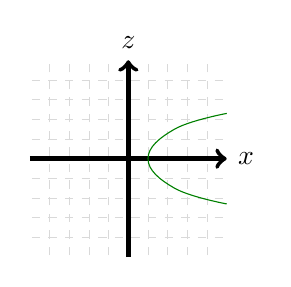
\begin{tikzpicture}[scale=0.25]
                \draw[help lines, color=gray!30, dashed] (-4.9,-4.9) grid (4.9,4.9);
                \draw[->, ultra thick] (-5,0) -- (5,0) node[right]{$x$};
                \draw[->, ultra thick] (0,-5) -- (0,5) node[above]{$z$};
                \draw[green!50!black] plot[smooth, tension=0.7] coordinates {(5,2.3) (2.35,1.5) (1,0) (2.35,-1.5) (5,-2.3)};
            \end{tikzpicture}
            \par\egroup

            Rotating this about the $z$ axis gives

            \bgroup\centering
            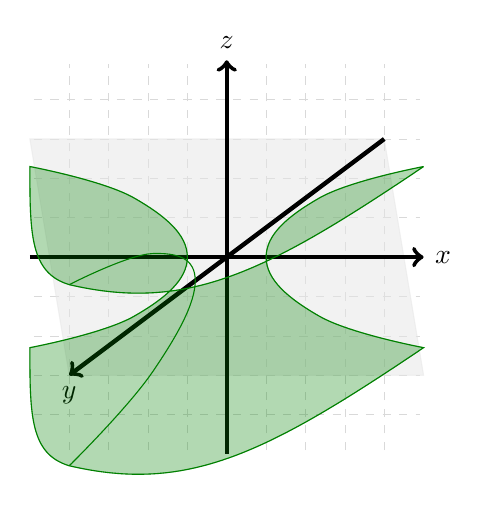
\begin{tikzpicture}[scale=0.5]
                \draw[help lines, color=gray!30, dashed] (-4.9,-4.9) grid (4.9,4.9);
                \filldraw[white!90!black, opacity=0.5] (5,-3) -- (4,3) -- (-5,3) -- (-4,-3) -- cycle;
                \draw[->, ultra thick] (-5,0) -- (5,0) node[right]{$x$};
                \draw[->, ultra thick] (0,-5) -- (0,5) node[above]{$z$};
                \draw[->, ultra thick] (4,3) -- (-4,-3) node[below]{$y$};
                %\draw[green!50!black] plot[smooth, tension=0.7] coordinates {(5,2.3) (2.35,1.5) (1,0) (2.35,-1.5) (5,-2.3)};
                %\draw[green!50!black] plot[smooth, tension=0.7] coordinates {(-5,2.3) (-2.35,1.5) (-1,0) (-2.35,-1.5) (-5,-2.3)};
                \draw[green!50!black] plot[smooth, tension=0.7] coordinates {(-4,-0.7) (-1.88,0.09) (-0.8,-0.6) (-1.88, -2.91) (-4, -5.3)};
                %\filldraw[green!50!black,opacity=0.3] (5,2.3) .. controls (-1,1) and (-2,1) .. (-5,2.3) -- (-5,-2.3) .. controls (-2,-3.6) and (-1,-3.6) .. (5,-2.3) -- cycle;
                %\filldraw[green!50!black,opacity=0.3] plot[smooth, tension=0.7] coordinates {(5,2.3) (2.35,1.5) (1,0) (2.35,-1.5) (5,-2.3)} .. controls (-1,-3.6) and (-2,-3.6) .. (-5,-2.3) --
                %plot[smooth, tension=0.7] coordinates {(-5,-2.3) (-2.35,-1.5) (-1,0) (-2.35,1.5) (-5,2.3)} .. controls (-2,1) and (-1,1) .. (5,2.3);
                \filldraw[green!50!black,opacity=0.3] plot[smooth, tension=0.7] coordinates {(5,2.3) (2.35,1.5) (1,0) (2.35,-1.5) (5,-2.3)} .. controls (1,-5) and (-1,-6) .. (-4,-5.3)
                .. controls (-5,-5) and (-5,-4) .. (-5,-2.3) -- plot[smooth, tension=0.7] coordinates {(-5,-2.3) (-2.35,-1.5) (-1,0) (-2.35,1.5) (-5,2.3)} ..
                controls (-5,0.6) and (-5,-0.4) .. (-4,-0.7) .. controls (-1,-1.4) and (1,-0.4) .. (5,2.3);
                \draw[green!50!black] plot[smooth, tension=0.7] coordinates {(5,2.3) (2.35,1.5) (1,0) (2.35,-1.5) (5,-2.3)} .. controls (1,-5) and (-1,-6) .. (-4,-5.3)
                .. controls (-5,-5) and (-5,-4) .. (-5,-2.3) -- plot[smooth, tension=0.7] coordinates {(-5,-2.3) (-2.35,-1.5) (-1,0) (-2.35,1.5) (-5,2.3)} ..
                controls (-5,0.6) and (-5,-0.4) .. (-4,-0.7) .. controls (-1,-1.4) and (1,-0.4) .. (5,2.3);
            \end{tikzpicture}
            \par\egroup
            (This isn't perfect, the fill should fill into the rotated hyperbolic cosine graph, but I'm not really sure how to do that using Ti\textit{k}Z.
            Note that I did use Ti\textit{k}Z, not pgfplots.
            I computed coordinates on the curve, and then using Ti\textit{k}Z interpolated a curve through them.)
    \eenum

\eblank

\bexerc

    Find the mean curvature at every point on the surface from the previous questions in two ways: via direct computation and via the Laplacian.

\eexerc

\bblank

    \benum
        \item We know the mean curvature is $H=\frac12\traceof S=0$.
        \item Our parameterization is an isomothermic parameterization, as $g$ is a scalar matrix ($f=\cosh$).
            Thus $\Delta\sigma=-2\cosh^2(t)H\rho$, and since
            \[ \Delta\sigma = \sigma_{11} + \sigma_{22} = 0 \]
            this means that $H=0$.
    \eenum

\eblank

\bexerc

    Give an example for a surface which satisfies:
    \benum
        \item There is no point which has negative Gaussian curvature.
        \item Some points have negative Gaussian curvature, but not all of them.
        \item Every point has negative Gaussian curvature, and the curvature is not constant.
    \eenum

\eexerc

\bblank

    \benum
        \item Let the surface be a paraboloid,
            \[ \sigma(u,v) = (u,v,u^2+v^2) \]
            this is the graph of the function $f(u,v)=u^2+v^2$.
            Thus it has Gaussian curvature:
            \[ K = \frac{f_{uu}f_{vv}-f_{uv}^2}{(1+f_u^2+f_v^2)^2} = \frac4{(1+4u^2+4v^2)^2} \]
            and this is always positive.

        \item Let the surface be given by the graph of $f(u,v)=u^3+v^3$,
            \[ \sigma(u,v) = (u,v,u^3+v^3) \]
            Then its Gaussian curvature is
            \[ K = \frac{f_{uu}f_{vv}-f_{uv}^2}{(1+f_u^2+f_v^2)^2} = \frac{36uv}{(1+9u^4+9v^4)^2} \]
            This is not always negative or positive (when $u$ and $v$ have the same sign, it is positive, when they have differing signs the curvature is negative).

        \item Let us alter the example we gave for the first question, we want $f_{uu}f_{vv}$ to be negative, so let $f(u,v)=u^2-v^2$.
            And $\sigma$ is the graph of $f$,
            \[ \sigma(u,v) = (u,v,u^2-v^2) \]
            This has the Gaussian curvature
            \[ K = \frac{f_{uu}f_{vv}-f_{uv}^2}{(1+f_u^2+f_v^2)^2} = -\frac4{(1+4u^2+4v^2)^2} \]
            This is always negative, and not constant.
    \eenum

\eblank

\bexerc

    Show that the Enneper surface is a minimal surface,
    \[ \sigma(u,v) = \parens{u-\frac13u^3+uv^2,-v+\frac13v^3-vu^2,u^2-v^2} \]

\eexerc

\bblank

    Let us compute the partial derivatives of $\sigma$:
    \begin{align*}
        \sigma_1 &= \parens{1-u^2+v^2,-2uv,2u} \\
        \sigma_2 &= \parens{2uv,-1+v^2-u^2,-2v} \\
        \sigma_{11} &= \parens{-2u,-2v,2} \\
        \sigma_{12} = \sigma_{21} &= \parens{2v,-2u,0} \\
        \sigma_{22} &= \parens{2u,2v,-2}
    \end{align*}
    Then
    \begin{align*}
        g_{11} &= (1+u^2+v^2)^2 \\
        g_{12} = g_{21} &= 0 \\
        g_{22} &= (1+u^2+v^2)
    \end{align*}
    So the metric is equal to
    \[ g = (1+u^2+v^2)\pmat{1 & 0 \\ 0 & 1} \]
    This means that $\sigma$ is an isothermic parameterization.
    So in order to show that the surface is minimal, ie. that $H=0$, it is sufficient to show that the Laplacian of $\sigma$ is zero.
    And since
    \[ \Delta\sigma = \sigma_{11} + \sigma_{22} = (0,0,0) \]
    this is indeed the case.
    So the surface is indeed minimal.

\eblank

\bexerc

    Show that the Scherk surface is minimal,
    \[ \sigma(u,v) = \parens{u,v,\log\parens{\frac{\cos v}{\cos u}}} \]

\eexerc

\bblank

    We once again compute the partial derivatives of $\sigma$.
    \begin{align*}
        \sigma_1 &= \parens{1,0,-\tan u} \\
        \sigma_2 &= \parens{0,1,\tan v} \\
        \sigma_{11} &= \parens{0,0,-\frac1{\cos^2(u)}} \\
        \sigma_{12} = \sigma_{21} &= (0,0,0) \\
        \sigma_{22} &= \parens{0,0,\frac1{\cos^2(v)}}
    \end{align*}
    Thus we have that using $g_{ij}=\iprod{\sigma_i,\sigma_j}$,
    \[ g = \pmat{1+\tan^2(u) & -\tan(u)\tan(v) \\ -\tan(u)\tan(v) & 1+\tan^2(v)} \] 
    Notice that $\detof g=1+\tan^2(u)+\tan^2(v)$.
    Now, we will compute the unit normal, but first $\sigma_1\times\sigma_2$:
    \[ \sigma_1\times\sigma_2 = \det\pmat{e_1 & e_2 & e_3 \\ 1 & 0 & -\tan(u) \\ 0 & 1 & \tan(v)} = \pmat{\tan(u) \\ -\tan(v) \\ 1} \]
    Normalizing gives
    \[ \rho = \frac1{\sqrt{1+\tan^2(u)+\tan^2(v)}}\pmat{\tan(u) \\ -\tan(v) \\ 1} \]
    Now we will compute the second fundamental form, $B$, utilizing $b_{ij}=\iprod{\rho,\sigma_{ij}}$.
    \begin{align*}
        \iprod{\rho,\sigma_{11}} &= \frac1{\sqrt{1+\tan^2(u)+\tan^2(v)}}\cdot\parens{-\frac1{\cos^2(u)}} \\
        \iprod{\rho,\sigma_{12}} = \iprod{\rho,\sigma_{21}} &= 0 \\
        \iprod{\rho,\sigma_{22}} &= \frac1{\sqrt{1+\tan^2(u)+\tan^2(v)}}\cdot\frac1{\cos^2(v)}
    \end{align*}
    Thus
    \[ B = \frac1{\sqrt{\detof g}}\pmat{-\cos^{-2}(u) & 0 \\ 0 & \cos^{-2}(v)} \]
    And computing the adjugate and from that the inverse, we have that
    \[ g^{-1} = \frac1{\det g}\pmat{1+\tan^2(v) & \tan(u)\tan(v) \\ \tan(u)\tan(v) & 1+\tan^2(u)} \]
    And since $S=g^{-1}B$ we have
    \[ S = \frac1{\detof g^{1.5}}\pmat{-\cos^{-2}(u)\bigl(1+\tan^2(v)\bigr) & * \\ * & \cos^{-2}(v)\bigl(1+\tan^2(u)\bigr)} \]
    (We can ignore the coefficients which aren't on the diagonal since we are interested in $H=\frac12\traceof S$.)
    So we can now compute the mean curvature by $H=\frac12\traceof S$,
    \begin{multline*}
        \traceof S = -\frac1{\cos^2(u)} - \frac{\sin^2(v)}{\cos^2(u)\cos^(v)} + \frac1{\cos^2(v)} + \frac{\sin^2(u)}{\cos^2(u)\cos^2(v)} \\
        = \frac{-\cos^2(v)-\sin^2(v)+\cos^2(u)+\sin^2(u)}{\cos^2(u)\cos^2(v)} = \frac{-1+1}{\cos^2(u)\cos^2(v)} = 0
    \end{multline*}
    Thus $H=0$, so the surface is minimal, as required.

\eblank

\bexerc

    Compute the total curvature of
    \[ \alpha(t) = \bigl(\cos(2t),\,\sin(2t)\bigr) \]
    where $t\in[0,4\pi]$.

\eexerc

\bblank

    Let $\beta(t)=\alpha\parens{\frac t2}=(\cos(t),\sin(t))$ be a reparameterization of $\alpha$.
    Since $\alpha\colon[0,4\pi]\longto\bR^2$, and the preimage of $[0,4\pi]$ under $t\mapsto\frac t2$ is $[0,8\pi]$, we have that $\beta$'s domain is $[0,8\pi]$.
    Further notice that $\norm{\beta'}=1$ and so $\beta$ is $\alpha$'s natural parameterization.
    $\beta$ is the natural parameterization of the unit circle, and so its curvature is $\frac1R=1$.
    So
    \[ K = \int_0^{8\pi}1 = 8\pi \]

\eblank

\bexerc

    Let us focus on the \emph{Leminscate of Gerono}, the curve
    \[ \alpha(t) = \parens{\sin(t),\frac12\sin(2t)},\quad t\in[0,2\pi] \]
    \benum
        \item Sketch a graph of $\alpha$.
        \item Using the sketch estimate $\alpha$'s total curvature.
        \item Find the total curvature of $\alpha$.
    \eenum

\eexerc

\bblank

    \benum
        \item Let us notice that
            \[ \alpha(\theta+\pi) = \parens{\sin(\theta+\pi),\frac12\sin(2\theta+2\pi)} = \parens{-\sin(\theta),\frac12\sin(2\theta)} \]
            and
            \[ \alpha(\pi-\theta) = \parens{\sin(\pi-\theta),\frac12\sin(2\pi-2\theta)} = \parens{\sin(\theta),-\frac12\sin(2\theta)} \]
            Meaning there is an antisymmetry around $\pi$, as $\alpha(\pi-\theta)$ reflects $\alpha(\theta)$ across the $x$ axis, and $\alpha(\pi+\theta)$ reflexts $\alpha(\theta)$ across the $y$ axis.
            This means that the curve is symmetric across the $x$ and $y$ axis, so it is sufficient to draw one quarter of the curve (ie for $0\leq t\leq\frac\pi2$).
            So let us sample the points where $t=\frac\pi8a$ where $a=0,\dots,4$.
            \[ \alpha(0) = 0,\quad \alpha\parens{\frac\pi8}=(0.383,0.354),\quad \alpha\parens{\frac\pi4} = \parens{\frac1{\sqrt2},0.5},\quad \alpha\parens{\frac{3\pi}8}=(0.924,0.354),\quad
            \alpha\parens{\frac\pi2}=(1,0) \]
            So interpolating a curve through these points and reflecting it across the $x$ and $y$ axes gives the curve

            \bgroup\centering
            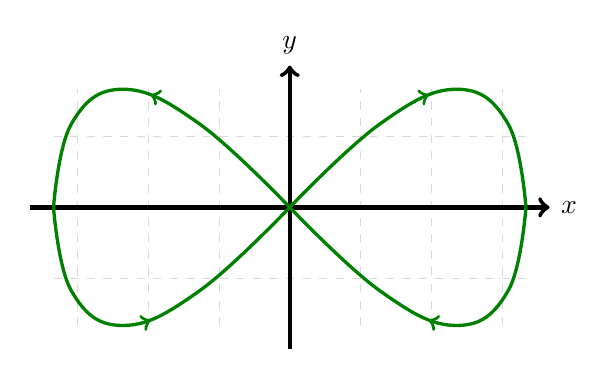
\begin{tikzpicture}[scale=3]
                \draw[help lines, color=gray!30, dashed] (-1,-0.5) grid[step=0.3] (1,0.5);
                \draw[->, ultra thick] (-1.1,0) -- (1.1,0) node[right]{$x$};
                \draw[->, ultra thick] (0,-0.6) -- (0,0.6) node[above]{$y$};
                \begin{scope}[green!50!black, very thick, decoration={
                        markings,
                        mark=at position 0.5 with {\arrow{>}}}
                    ]
                    \draw[postaction={decorate}] plot[smooth, tension=0.7] coordinates {(0,0) (0.383, 0.354) (0.707,0.5) (0.924,0.354) (1,0)};
                    \draw[postaction={decorate}] plot[smooth, tension=0.7] coordinates {(1,0) (0.924,-0.354) (0.707,-0.5) (0.383, -0.354) (0,0)};
                    \draw[postaction={decorate}] plot[smooth, tension=0.7] coordinates {(0,0) (-0.383, 0.354) (-0.707,0.5) (-0.924,0.354) (-1,0)};
                    \draw[postaction={decorate}] plot[smooth, tension=0.7] coordinates {(-1,0) (-0.924,-0.354) (-0.707,-0.5) (-0.383, -0.354) (0,0)};
                \end{scope}
            \end{tikzpicture}
            \par\egroup

        \item Notice that the left half of the curve is reflected onto the right half.
            But while the left half moves clockwise, the right half moves counterclockwise.
            So the total curvature of the left half is equal to $-1$ times the total curvature of the right half, as they are symmetric but move in different directions.
            So the total curvature of the curve as a whole should be zero.

        \item Now, since
            \[ \alpha'(t) = (\cos t,\cos(2t)),\quad \alpha''(t) = -(\sin t,2\sin(2t)) \]
            And the curvature is given by
            \[ \kappa = \frac{\alpha_2''\alpha'_1 - \alpha'_2\alpha''_1}{\bigl((\alpha'_1)^2+(\alpha'_2)^2\bigr)^{1.5}} = \frac{-2\sin(2t)\cos(t)-\cos(2t)\sin(t)}{(\cos^2(t)+\cos^2(2t))^{1.5}} \]
            Thus the total curvature is given by
            \[ K = \int_0^{2\pi}\kappa(t) = \int_0^{2\pi}\frac{-2\sin(2t)\cos(t)-\cos(2t)\sin(t)}{(\cos^2(t)+\cos^2(2t))^{1.5}} \]
            But notice that
            \[ \kappa(\pi+t) = \frac{2\sin(2t)\cos(t)+\cos(2t)\sin(t)}{(\cos^2(t)+\cos^2(2t))^{1.5}} = -\kappa(t) \]
            And
            \[ \kappa(\pi-t) = \frac{-2\sin(2t)\cos(t)-\cos(2t)\sin(t)}{(\cos^2(t)+\cos^2(2t))^{1.5}} = \kappa(t) \]
            So $\kappa$ is antisymmetric around $\pi$, thus integrating on a symmetric domain around $\pi$, for example $[0,2\pi]$ will equal zero.
            Meaning
            \[ K = \int_0^{2\pi}\kappa = 0 \]
            as required.
    \eenum

\eblank

\bexerc

    Show that if $\gamma$ is a regular Jordan curve then the radial vector is orthogonal to the tangent vector of $\gamma$ at its closest point to the origin.

\eexerc

\bblank

    The distance between the radius vector ($\gamma(t)$) and the origin is given by $\norm{\gamma(t)}$, and since this is positive, it has a minimum if and only if
    $\norm{\gamma(t)}=\iprod{\gamma(t),\gamma(t)}$ has a minimum.
    Let $f(t)=\iprod{\gamma(t),\gamma(t)}$, so we are trying to show that at a minimum point of $f$, $\gamma(t)$ (the radial vector) and $\gamma'(t)$ (the tangent vector) are orthogonal.
    At a minimum, the derivative of $f$ becomes zero, and
    \[ f'(t) = \iprod{\gamma'(t),\gamma(t)} + \iprod{\gamma(t),\gamma'(t)} = 2\iprod{\gamma(t),\gamma'(t)} \]
    So if $p=f(t)$ is the closest point to the origin then $f'(t)=0$ and so $\iprod{\gamma(t),\gamma'(t)}=0$, meaning $\gamma(t)$ and $\gamma'(t)$ are orthogonal, as required.

\eblank

\end{document}

